\documentclass{FR16} 
\setlength{\parindent}{3em}
\setlength{\parskip}{1em}
\renewcommand{\baselinestretch}{1.5}
\begin{document}


\maketitle

\tableofcontents
\newpage

\section{Introducción}
El objetivo de este proyecto es crear un sistema para gestionar el funcionamiento del refugio de animales para servicios públicos o para empresas privadas. El trabajo propuesto se centra en el desarrollo de bases de datos, aplicación y documentación para ellos. El sistema es una aplicación Java que permite interactuar con la Base de datos Oracle.

Este aplicación permite llevar un registro de los animales ingresados, sus vacunas y procedimientos. También se mantiene un registro de las familias que toman el animal del refugio o lo devuelven.

Las herramientas de desarrollo fueron Oracle Database Express, el lenguaje pl/SQL para la creación de bases de datos y el lenguaje de programación Java.

\newpage

\section{Descripción del contexto y requisitos funcionales y no funcionales}
\subsection{Descripción del contexto}
\begin{center}
Descripción del contexto
\end{center}


\subsection{Requisitos funcionales y no funcionales}
\begin{center}
Requisitos funcionales
\end{center}

\newpage

\section{Diseño lógico y físico del sistema}
\subsection{Diagrama de clases}
\begin{figure}[H]
\centering
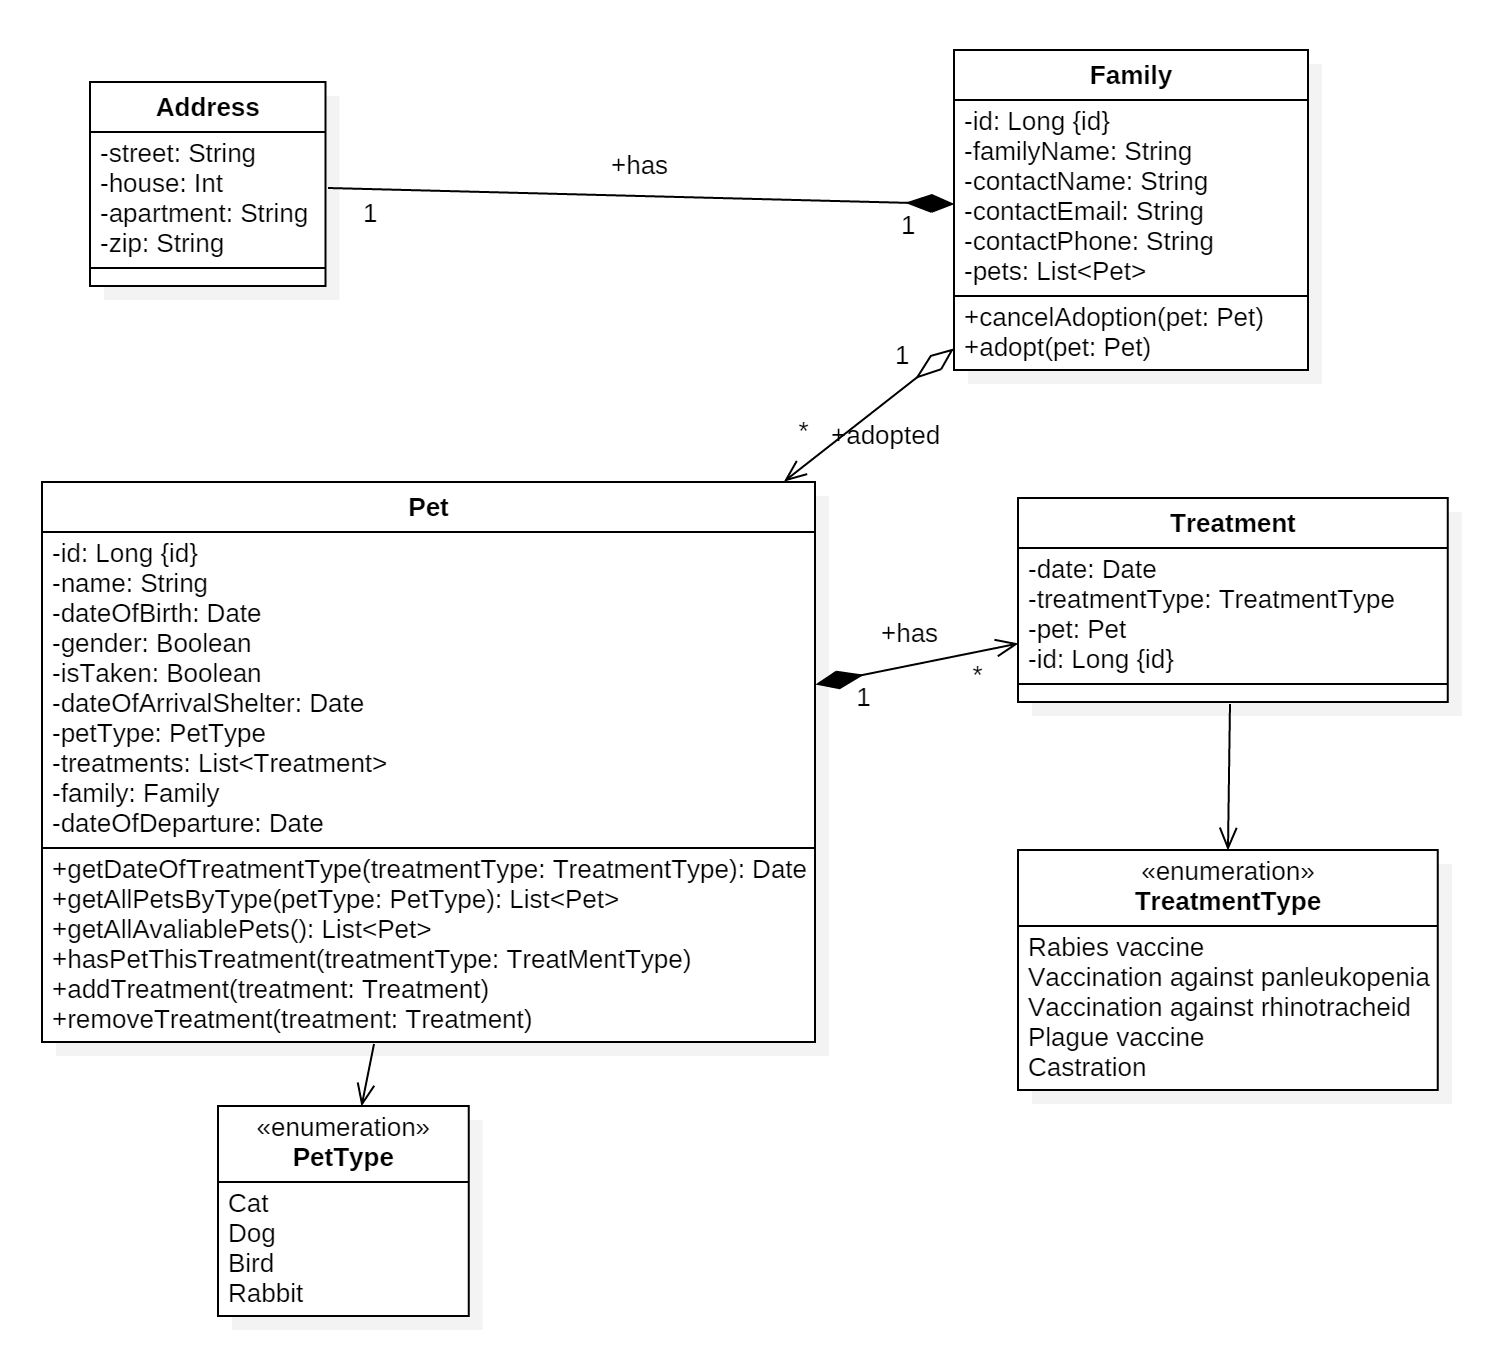
\includegraphics[width=1\textwidth]{Logical View.png}
\caption{\label{fig:1}Diagrama de clases.}
\end{figure}

\newpage

El \textbf{diagrama de clases} para esta aplicación consta de 4 clases y 2 enumeraciones. La tabla 'Pet' almacena toda la información relacionada con ella. La tabla está vinculada a la tabla 'Treatment' por la relación composición, que almacena todos los procedimientos en curso.Cada tipo de 'Treatment' tiene 'TreatmentType'. También hay una relación con la tabla 'Familia' agregación, ya que no todos en la tabla 'Pet'   tienen 'Family'. Cada mascota tiene un tipo que existe en la enumeración 'PetType'.

\subsection{Esquema lógico O / R específico}
\begin{center}
Esquema lógico O / R específico
\end{center}


\subsection{Diseño físico}
\begin{center}
Physical desing
\end{center}
\newpage

\section{Desarrollo del sistema}
\subsection{Disparadores}
Los \textbf{disparadores} (o triggers) son bloques de código PL/SQL asociados a una tabla y que se ejecutan automáticamente como reacción a una operación DML específica (INSERT, UPDATE o DELETE) sobre dicha tabla.

En definitiva, los disparadores son eventos a nivel de tabla que se ejecutan automáticamente cuando se realizan ciertas operaciones sobre la tabla.

\begin{lstlisting}[language=Sql]
CREATE {OR REPLACE} TRIGGER nombre_disp
  [BEFORE|AFTER]
  [DELETE|INSERT|UPDATE {OF columnas}] 
  [ OR [DELETE|INSERT|UPDATE {OF columnas}]...]
  ON tabla
  [FOR EACH ROW [WHEN condicion disparo]]
[DECLARE]
  -- Declaración de variables locales
BEGIN
  -- Instrucciones de ejecución
[EXCEPTION]
  -- Instrucciones de excepción
END;
\end{lstlisting}
\subsection{Paquete}

Como su nombre infiere, es una envoltura que agrupa un conjunto de objectos relacionados hasta cierto punto. Enfocado en PL/SQL un \textbf{paquete} puede ser definido como:

Un objeto de esquema que agrupa objectos relacionados(PL/SQL types, variables, y subprogramas) de forma lógica. Por lo general los Paquetes contienen dos partes, una especificación y un cuerpo, aunque a veces el cuerpo es innecesario. La especificación es donde se define la interfaz de tus aplicaciones; en la cual se declaran los tipos(types), variables, constantes, excepciones, cursores y subprogramas. En el cuerpo es donde se le da uso a los objectos antes declarados, ademas de ser donde se desarrolla/implementa la lógica completa del paquete.

\begin{lstlisting}[language=Sql]
--Especificación
CREATE [ OR REPLACE ] PACKAGE [ schema. ]package
   [ invoker_rights_clause ]
   { IS | AS } pl/sql_package_spec;

--Cuerpo
CREATE [ OR REPLACE ] PACKAGE BODY [ schema. ]package
   { IS | AS } pl/sql_package_body;
\end{lstlisting}
\newpage

\section{Conclusiones}
\begin{center}
Conclusiones
\end{center}

\newpage
\begin{thebibliography}{9}
\bibitem{churchel}
Charchel, Clare, \emph{Beginning database desing}. APRESS, Second edition, 2007
\end{thebibliography}

\end{document}